\clearpage
\section{Vyhodnocení}
\def\projekt{TAČR SIGMA\_DC3 \enquote{Telemedicínské samovyšetření řeči a paměti pro rychlou detekci kognitivních poruch metodami strojového učení}}
Posledním krokem bylo ověření funkčnosti navrženého a implementovaného systému.
K tomu bylo potřeba získat vhodná data, konkrétně obrázek a k němu přirozené popisy, pokud možnost v textové podobě.
Tato data byla získána z projektu \projekt.

Popisovanou scénou byla kresba zobrazená na Obrázku~\ref{fig:summer}.
K tomuto obrázku bylo k dispozici několik přepisů, které byly použité pro účely testování.

Referenční popis daného obrázku, stejně jako SPGF gramatika a ztrátová tabulka,
byly vytvořené autorem této práce a nikoli expertem z oboru, odkud pocházejí nasbíraná data.

Hodnoty ve ztrátové tabulce je tedy třeba chápat jako ilustrační a ve výsledcích je možné srovnávat pouze relativní ztráty,
nelze dělat smysluplné závěry z konkrétních hodnot.
To však nepředstavuje problém, protože cílem zde bylo ověřit funkčnost navrženého systému, na což ilustrační hodnoty postačují.

Vytvořený referenční popis Obrázku~\ref{fig:summer} obsahuje 69 objektů a 37 vazeb mezi nimi a je možné jej prozkoumat spolu se sestavenou SPGF gramatikou u zdrojových kódů.
Ztrátová tabulka použitá při testování je na Výpisu~\ref{lst:loss_table_example}.

% \begin{lstlisting}[
	% there are many more options of styling, see the official documentation, these are just the defaults I like
	frame=single, % make single-line frame around the verbatim
	framesep=2mm, % put some more spacing between the frame and text
	aboveskip=5mm, % put some more space above the box
	basicstyle={\linespread{0.9}\small\ttfamily}, % use typewriter (monospace) font
	caption={Ztrátová tabulka použitá při testování}, % set the caption text
	captionpos=b, % put the caption at the bottom (b) or top (t) or both (bt)
	label={lst:loss_table_example}, % label to be referenced via \ref{}
	numbers=left, % line numbers on the left
	numberstyle={\scriptsize\ttfamily\color{black!60}}, % the style for line numbers
	escapeinside={<@}{@>} % between those sequences are command evaluated
]
<@\textcolor[HTML]{FF1010}{\texttt{\{}}@>
<@\textcolor[HTML]{000000}{\texttt{\ \ }}@><@\textcolor[HTML]{255CFF}{\texttt{"missing\_objects"}}@><@\textcolor[HTML]{1041FF}{\texttt{:}}@><@\textcolor[HTML]{000000}{\texttt{\ }}@><@\textcolor[HTML]{DE6F10}{\texttt{3}}@><@\textcolor[HTML]{1041FF}{\texttt{,}}@>
<@\textcolor[HTML]{000000}{\texttt{\ \ }}@><@\textcolor[HTML]{255CFF}{\texttt{"missing\_attributes"}}@><@\textcolor[HTML]{1041FF}{\texttt{:}}@><@\textcolor[HTML]{000000}{\texttt{\ }}@><@\textcolor[HTML]{DE6F10}{\texttt{1}}@><@\textcolor[HTML]{1041FF}{\texttt{,}}@>
<@\textcolor[HTML]{000000}{\texttt{\ \ }}@><@\textcolor[HTML]{255CFF}{\texttt{"missing\_triplets"}}@><@\textcolor[HTML]{1041FF}{\texttt{:}}@><@\textcolor[HTML]{000000}{\texttt{\ }}@><@\textcolor[HTML]{DE6F10}{\texttt{2}}@><@\textcolor[HTML]{1041FF}{\texttt{,}}@>
<@\textcolor[HTML]{000000}{\texttt{\ \ }}@><@\textcolor[HTML]{255CFF}{\texttt{"numberless\_penalty"}}@><@\textcolor[HTML]{1041FF}{\texttt{:}}@><@\textcolor[HTML]{000000}{\texttt{\ }}@><@\textcolor[HTML]{DE6F10}{\texttt{0.5}}@><@\textcolor[HTML]{1041FF}{\texttt{,}}@>
<@\textcolor[HTML]{000000}{\texttt{\ \ }}@><@\textcolor[HTML]{255CFF}{\texttt{"wrong\_values"}}@><@\textcolor[HTML]{1041FF}{\texttt{:}}@><@\textcolor[HTML]{000000}{\texttt{\ }}@><@\textcolor[HTML]{DE6F10}{\texttt{2}}@><@\textcolor[HTML]{1041FF}{\texttt{,}}@>
<@\textcolor[HTML]{000000}{\texttt{\ \ }}@><@\textcolor[HTML]{255CFF}{\texttt{"missing\_objects\_override"}}@><@\textcolor[HTML]{1041FF}{\texttt{:}}@><@\textcolor[HTML]{000000}{\texttt{\ }}@><@\textcolor[HTML]{FF1010}{\texttt{[}}@>
<@\textcolor[HTML]{000000}{\texttt{\ \ \ \ }}@><@\textcolor[HTML]{FF1010}{\texttt{[}}@><@\textcolor[HTML]{418310}{\texttt{"person"}}@><@\textcolor[HTML]{1041FF}{\texttt{,}}@><@\textcolor[HTML]{000000}{\texttt{\ }}@><@\textcolor[HTML]{DE6F10}{\texttt{5}}@><@\textcolor[HTML]{FF1010}{\texttt{]}}@><@\textcolor[HTML]{1041FF}{\texttt{,}}@>
<@\textcolor[HTML]{000000}{\texttt{\ \ \ \ }}@><@\textcolor[HTML]{FF1010}{\texttt{[}}@><@\textcolor[HTML]{418310}{\texttt{"animal"}}@><@\textcolor[HTML]{1041FF}{\texttt{,}}@><@\textcolor[HTML]{000000}{\texttt{\ }}@><@\textcolor[HTML]{DE6F10}{\texttt{4}}@><@\textcolor[HTML]{FF1010}{\texttt{]}}@><@\textcolor[HTML]{1041FF}{\texttt{,}}@>
<@\textcolor[HTML]{000000}{\texttt{\ \ \ \ }}@><@\textcolor[HTML]{FF1010}{\texttt{[}}@><@\textcolor[HTML]{418310}{\texttt{"environment"}}@><@\textcolor[HTML]{1041FF}{\texttt{,}}@><@\textcolor[HTML]{000000}{\texttt{\ }}@><@\textcolor[HTML]{DE6F10}{\texttt{1}}@><@\textcolor[HTML]{FF1010}{\texttt{]}}@>
<@\textcolor[HTML]{000000}{\texttt{\ \ }}@><@\textcolor[HTML]{FF1010}{\texttt{]}}@><@\textcolor[HTML]{1041FF}{\texttt{,}}@>
<@\textcolor[HTML]{000000}{\texttt{\ \ }}@><@\textcolor[HTML]{255CFF}{\texttt{"missing\_attributes\_override"}}@><@\textcolor[HTML]{1041FF}{\texttt{:}}@><@\textcolor[HTML]{000000}{\texttt{\ }}@><@\textcolor[HTML]{FF1010}{\texttt{[}}@>
<@\textcolor[HTML]{000000}{\texttt{\ \ \ \ }}@><@\textcolor[HTML]{FF1010}{\texttt{[}}@><@\textcolor[HTML]{418310}{\texttt{"action"}}@><@\textcolor[HTML]{1041FF}{\texttt{,}}@><@\textcolor[HTML]{000000}{\texttt{\ }}@><@\textcolor[HTML]{DE6F10}{\texttt{1.5}}@><@\textcolor[HTML]{FF1010}{\texttt{]}}@><@\textcolor[HTML]{1041FF}{\texttt{,}}@>
<@\textcolor[HTML]{000000}{\texttt{\ \ \ \ }}@><@\textcolor[HTML]{FF1010}{\texttt{[}}@><@\textcolor[HTML]{418310}{\texttt{"state"}}@><@\textcolor[HTML]{1041FF}{\texttt{,}}@><@\textcolor[HTML]{000000}{\texttt{\ }}@><@\textcolor[HTML]{DE6F10}{\texttt{0.5}}@><@\textcolor[HTML]{FF1010}{\texttt{]}}@>
<@\textcolor[HTML]{000000}{\texttt{\ \ }}@><@\textcolor[HTML]{FF1010}{\texttt{]}}@><@\textcolor[HTML]{1041FF}{\texttt{,}}@>
<@\textcolor[HTML]{000000}{\texttt{\ \ }}@><@\textcolor[HTML]{255CFF}{\texttt{"missing\_triplets\_override"}}@><@\textcolor[HTML]{1041FF}{\texttt{:}}@><@\textcolor[HTML]{000000}{\texttt{\ }}@><@\textcolor[HTML]{FF1010}{\texttt{[}}@><@\textcolor[HTML]{FF1010}{\texttt{[}}@><@\textcolor[HTML]{418310}{\texttt{"falling\ into"}}@><@\textcolor[HTML]{1041FF}{\texttt{,}}@><@\textcolor[HTML]{000000}{\texttt{\ }}@><@\textcolor[HTML]{DE6F10}{\texttt{5}}@><@\textcolor[HTML]{FF1010}{\texttt{]}}@><@\textcolor[HTML]{FF1010}{\texttt{]}}@><@\textcolor[HTML]{1041FF}{\texttt{,}}@>
<@\textcolor[HTML]{000000}{\texttt{\ \ }}@><@\textcolor[HTML]{255CFF}{\texttt{"wrong\_values\_override"}}@><@\textcolor[HTML]{1041FF}{\texttt{:}}@><@\textcolor[HTML]{000000}{\texttt{\ }}@><@\textcolor[HTML]{FF1010}{\texttt{[}}@>
<@\textcolor[HTML]{000000}{\texttt{\ \ \ \ }}@><@\textcolor[HTML]{FF1010}{\texttt{\{}}@>
<@\textcolor[HTML]{000000}{\texttt{\ \ \ \ \ \ }}@><@\textcolor[HTML]{255CFF}{\texttt{"attribute"}}@><@\textcolor[HTML]{1041FF}{\texttt{:}}@><@\textcolor[HTML]{000000}{\texttt{\ }}@><@\textcolor[HTML]{418310}{\texttt{"color"}}@><@\textcolor[HTML]{1041FF}{\texttt{,}}@>
<@\textcolor[HTML]{000000}{\texttt{\ \ \ \ \ \ }}@><@\textcolor[HTML]{255CFF}{\texttt{"default"}}@><@\textcolor[HTML]{1041FF}{\texttt{:}}@><@\textcolor[HTML]{000000}{\texttt{\ }}@><@\textcolor[HTML]{DE6F10}{\texttt{0.5}}@><@\textcolor[HTML]{1041FF}{\texttt{,}}@>
<@\textcolor[HTML]{000000}{\texttt{\ \ \ \ \ \ }}@><@\textcolor[HTML]{255CFF}{\texttt{"overrides"}}@><@\textcolor[HTML]{1041FF}{\texttt{:}}@><@\textcolor[HTML]{000000}{\texttt{\ }}@><@\textcolor[HTML]{FF1010}{\texttt{[}}@>
<@\textcolor[HTML]{000000}{\texttt{\ \ \ \ \ \ \ \ }}@><@\textcolor[HTML]{FF1010}{\texttt{[}}@><@\textcolor[HTML]{FF1010}{\texttt{[}}@><@\textcolor[HTML]{418310}{\texttt{"white"}}@><@\textcolor[HTML]{1041FF}{\texttt{,}}@><@\textcolor[HTML]{000000}{\texttt{\ }}@><@\textcolor[HTML]{418310}{\texttt{"yellow"}}@><@\textcolor[HTML]{1041FF}{\texttt{,}}@><@\textcolor[HTML]{000000}{\texttt{\ }}@><@\textcolor[HTML]{418310}{\texttt{"pink"}}@><@\textcolor[HTML]{FF1010}{\texttt{]}}@><@\textcolor[HTML]{1041FF}{\texttt{,}}@><@\textcolor[HTML]{000000}{\texttt{\ }}@><@\textcolor[HTML]{DE6F10}{\texttt{0.3}}@><@\textcolor[HTML]{FF1010}{\texttt{]}}@><@\textcolor[HTML]{1041FF}{\texttt{,}}@>
<@\textcolor[HTML]{000000}{\texttt{\ \ \ \ \ \ \ \ }}@><@\textcolor[HTML]{FF1010}{\texttt{[}}@><@\textcolor[HTML]{FF1010}{\texttt{[}}@><@\textcolor[HTML]{418310}{\texttt{"red"}}@><@\textcolor[HTML]{1041FF}{\texttt{,}}@><@\textcolor[HTML]{000000}{\texttt{\ }}@><@\textcolor[HTML]{418310}{\texttt{"blue"}}@><@\textcolor[HTML]{1041FF}{\texttt{,}}@><@\textcolor[HTML]{000000}{\texttt{\ }}@><@\textcolor[HTML]{418310}{\texttt{"green"}}@><@\textcolor[HTML]{1041FF}{\texttt{,}}@><@\textcolor[HTML]{000000}{\texttt{\ }}@><@\textcolor[HTML]{418310}{\texttt{"yellow"}}@><@\textcolor[HTML]{FF1010}{\texttt{]}}@><@\textcolor[HTML]{1041FF}{\texttt{,}}@><@\textcolor[HTML]{000000}{\texttt{\ }}@><@\textcolor[HTML]{DE6F10}{\texttt{0.8}}@><@\textcolor[HTML]{FF1010}{\texttt{]}}@>
<@\textcolor[HTML]{000000}{\texttt{\ \ \ \ \ \ }}@><@\textcolor[HTML]{FF1010}{\texttt{]}}@>
<@\textcolor[HTML]{000000}{\texttt{\ \ \ \ }}@><@\textcolor[HTML]{FF1010}{\texttt{\}}}@><@\textcolor[HTML]{1041FF}{\texttt{,}}@>
<@\textcolor[HTML]{000000}{\texttt{\ \ \ \ }}@><@\textcolor[HTML]{FF1010}{\texttt{\{}}@>
<@\textcolor[HTML]{000000}{\texttt{\ \ \ \ \ \ }}@><@\textcolor[HTML]{255CFF}{\texttt{"attribute"}}@><@\textcolor[HTML]{1041FF}{\texttt{:}}@><@\textcolor[HTML]{000000}{\texttt{\ }}@><@\textcolor[HTML]{418310}{\texttt{"action"}}@><@\textcolor[HTML]{1041FF}{\texttt{,}}@>
<@\textcolor[HTML]{000000}{\texttt{\ \ \ \ \ \ }}@><@\textcolor[HTML]{255CFF}{\texttt{"default"}}@><@\textcolor[HTML]{1041FF}{\texttt{:}}@><@\textcolor[HTML]{000000}{\texttt{\ }}@><@\textcolor[HTML]{DE6F10}{\texttt{1.5}}@><@\textcolor[HTML]{1041FF}{\texttt{,}}@>
<@\textcolor[HTML]{000000}{\texttt{\ \ \ \ \ \ }}@><@\textcolor[HTML]{255CFF}{\texttt{"overrides"}}@><@\textcolor[HTML]{1041FF}{\texttt{:}}@><@\textcolor[HTML]{000000}{\texttt{\ }}@><@\textcolor[HTML]{FF1010}{\texttt{[}}@>
<@\textcolor[HTML]{000000}{\texttt{\ \ \ \ \ \ \ \ }}@><@\textcolor[HTML]{FF1010}{\texttt{[}}@><@\textcolor[HTML]{FF1010}{\texttt{[}}@><@\textcolor[HTML]{418310}{\texttt{"sitting"}}@><@\textcolor[HTML]{1041FF}{\texttt{,}}@><@\textcolor[HTML]{000000}{\texttt{\ }}@><@\textcolor[HTML]{418310}{\texttt{"reading"}}@><@\textcolor[HTML]{FF1010}{\texttt{]}}@><@\textcolor[HTML]{1041FF}{\texttt{,}}@><@\textcolor[HTML]{000000}{\texttt{\ }}@><@\textcolor[HTML]{DE6F10}{\texttt{0.8}}@><@\textcolor[HTML]{FF1010}{\texttt{]}}@><@\textcolor[HTML]{1041FF}{\texttt{,}}@>
<@\textcolor[HTML]{000000}{\texttt{\ \ \ \ \ \ \ \ }}@><@\textcolor[HTML]{FF1010}{\texttt{[}}@><@\textcolor[HTML]{FF1010}{\texttt{[}}@><@\textcolor[HTML]{418310}{\texttt{"fishing"}}@><@\textcolor[HTML]{1041FF}{\texttt{,}}@><@\textcolor[HTML]{000000}{\texttt{\ }}@><@\textcolor[HTML]{418310}{\texttt{"sitting"}}@><@\textcolor[HTML]{FF1010}{\texttt{]}}@><@\textcolor[HTML]{1041FF}{\texttt{,}}@><@\textcolor[HTML]{000000}{\texttt{\ }}@><@\textcolor[HTML]{DE6F10}{\texttt{0.7}}@><@\textcolor[HTML]{FF1010}{\texttt{]}}@>
<@\textcolor[HTML]{000000}{\texttt{\ \ \ \ \ \ }}@><@\textcolor[HTML]{FF1010}{\texttt{]}}@>
<@\textcolor[HTML]{000000}{\texttt{\ \ \ \ }}@><@\textcolor[HTML]{FF1010}{\texttt{\}}}@>
<@\textcolor[HTML]{000000}{\texttt{\ \ }}@><@\textcolor[HTML]{FF1010}{\texttt{]}}@>
<@\textcolor[HTML]{FF1010}{\texttt{\}}}@>

\end{lstlisting}

V Tabulce~\ref{tab:exmple_extracts} je několik vět z prvního přepisu, k nimž je vypsána množina extrahovaných objektů $\mathcal{O}$,
množina extrahovaných atributů $\mathcal A$ a množina extrahovaných vazeb $\mathcal V$.
Jak je možné na těchto ukázkách vidět, tak navržený systém je schopen z přirozeného textu extrahovat očekávané sémantické informace.
Dalším pozitivním faktem je to, že všechny extrahované informace jsou skutečně obsažené v původních promluvách a tudíž lze usoudit, že filtrační
algoritmus pro odstranění falešných detekcí funguje správně.

\begin{table}[H]
	\centering

	\def\objone{\begin{tabular}{l}
			water  \\[-1mm]
			people \\[-1mm]
			animals
		\end{tabular}}

	\def\objtwo{\begin{tabular}{l}
			woman   \\[-1mm]
			lounger \\[-1mm]
			book    \\[-1mm]
			parasol
		\end{tabular}}

	\def\objthree{\begin{tabular}{l}
			blanket \\[-1mm]
			basket
		\end{tabular}}

	\def\objfour{\begin{tabular}{l}
			girl, shorts, \\[-1mm]
			swimsuit \#1  \\[-1mm]
			boy, cap      \\[-1mm]
			tshirt
		\end{tabular}}

	\def\attrone{\begin{tabular}{l}
			people: count = 5
		\end{tabular}}

	\def\attrtwo{---}

	\def\attrthree{---}

	\def\attrfour{\begin{tabular}{l}
			girl: hairstyle = ponytail \\[-1mm]
			tshirt: pattern = striped
		\end{tabular}}

	\def\tripone{\begin{tabular}{l}
			---
		\end{tabular}}
	\def\triptwo{woman reading book}
	\def\tripthree{---}
	\def\tripfour{\begin{tabular}{l}
			% girl \to\ wearing \to\ swimsuit \#1 \\[-1mm]
			% boy \to\ wearing \to\ cap
			girl wearing swimsuit \#1 \\[-1mm]
			boy wearing cap
		\end{tabular}}

	\def\senone{\emph{na břehu rybníka je pět osob a několik zvířat}}
	\def\sentwo{\emph{vlevo sedí žena na lehátku čte si knihu pod slunečníkem}}
	\def\senthree{\emph{vedle sebe má rozprostřenou piknikovou deku s košíkem a s jídlem na piknik}}
	\def\senfour{\hspace{-1.5mm}\begin{tabular}{l}
			\emph{je to děvče s culíkem a v plavkách a chlapec s kšiltovkou a pruhovanym } \\[-1mm]
			\emph{tričkem a kraťasy}
		\end{tabular}}

	\begin{tabular}{|l|ccc|}
		\hline
		Věta 1                    & \multicolumn{3}{l|}{\senone}                                                                                            \\ \hline
		\multirow{2}{*}{Extrakty} & \multicolumn{1}{c|}{Objekty $\mathcal O_{1}$} & \multicolumn{1}{c|}{Atributy $\mathcal A_{1}$} & Vazby $\mathcal V_{1}$ \\ \cline{2-4}
		                          & \multicolumn{1}{l|}{\objone}                  & \multicolumn{1}{c|}{\attrone}                  & \tripone               \\ \hline
		\hline
		Věta 2                    & \multicolumn{3}{l|}{\sentwo}                                                                                            \\ \hline
		\multirow{2}{*}{Extrakty} & \multicolumn{1}{c|}{Objekty $\mathcal O_{2}$} & \multicolumn{1}{c|}{Atributy $\mathcal A_{2}$} & Vazby $\mathcal V_{2}$ \\ \cline{2-4}
		                          & \multicolumn{1}{l|}{\objtwo}                  & \multicolumn{1}{c|}{\attrtwo}                  & \triptwo               \\ \hline
		\hline
		Věta 3                    & \multicolumn{3}{l|}{\senthree}                                                                                          \\ \hline
		\multirow{2}{*}{Extrakty} & \multicolumn{1}{c|}{Objekty $\mathcal O_{3}$} & \multicolumn{1}{c|}{Atributy $\mathcal A_{3}$} & Vazby $\mathcal V_{3}$ \\ \cline{2-4}
		                          & \multicolumn{1}{l|}{\objthree}                & \multicolumn{1}{c|}{\attrthree}                & \tripthree             \\ \hline
		\hline
		Věta 4                    & \multicolumn{3}{l|}{\senfour}                                                                                           \\ \hline
		\multirow{2}{*}{Extrakty} & \multicolumn{1}{c|}{Objekty $\mathcal O_{4}$} & \multicolumn{1}{c|}{Atributy $\mathcal A_{4}$} & Vazby $\mathcal V_{4}$ \\ \cline{2-4}
		                          & \multicolumn{1}{l|}{\objfour}                 & \multicolumn{1}{c|}{\attrfour}                 & \tripfour              \\ \hline
	\end{tabular}
	\caption{Příklad konkrétních vět z nich extrahovaných entit}\label{tab:exmple_extracts}
\end{table}


V Tabulce~\ref{tab:exmple_extracts} lze dále pozorovat, že nejpočetnější kategorií ve větách jsou objekty, jejichž zachycení je nejjednodušší a především jich věty také obsahují nejvíce.
Dále lze pozorovat, že detekovaný objekt \emph{swimsuit \#1} ve čtvrté větě má u sebe přiřazené číslování (v popise se vyskytují dvoje plavky, jedny červené na dívce v pozadí
a jedny bílé na ženě na lehátku).
To je významné z toho důvodu, že to značí schopnost systému rozlišit objekty stejného typu, jak bylo popsáno v sekci~\ref{subsubsec:cislovani_objektu}.

Předpokladem pro kvalitní výstup je kvalitní referenční popis a SPGF gramatika.
Oba tyto faktory jsou zcela závislé na expertovi, který vytváří jak referenční popis, tak gramatiku použitou pro extrakci sémantiky z textu.

To může představovat problém ve smyslu vysokých počátečních nákladů, protože tvorba referenčního popisu a SPGF gramatiky
vyžaduje znalost zde navrženého formátu a může být pro lidského experta časově náročná.
Naopak výhodou zvoleného přístupu je ale možnost upravovat a vylepšovat jak referenční popis, tak SPGF gramatiku i v budoucnu,
protože oba tyto vstupy jsou navržené tak, aby byly čitelné člověkem a bylo možné je v případě potřeby kdykoli upravit.

Dále tento expertní přístup a manuální správa vstupních dat umožňuje přesnou kontrolu, na rozdíl od jiných přístupů, například neuronových sítí, jejichž funkce je spíše black-box a
potřeba provést detailní změny nebo přímo kontrolovat některé aspekty procesu jsou velmi obtížné.

Celé přepisy použité pro další testování a získání ilustračních výstupů jsou následující:
\begin{enumerate}
	\item \textbf{Přepis 1:} \\
	      \emph{Na břehu rybníka je pět osob a několik zvířat. Vlevo sedí žena na lehátku, čte si knihu
		      pod slunečníkem. Vedle sebe má rozprostřenou piknikovou deku s košíkem a s jídlem
		      na piknik. Opodál si hrají děti s míčem, hází si. Je to děvče s culíkem a v plavkách a
		      chlapec s kšiltovkou a pruhovanym tričkem a kraťasy. Na pravé straně sedí rybář,
		      který chytá ryby, má nahozený prut a vedle sebe podběrák. Před ním skáče žába
		      z kamene do rybníka. Mezi ženou a rybářem je uprostřed dítě, které vypadá, že padá
		      do rybníka, doufám, že ho někdo zachrání, že si ho někdo všimne. A vpředu vpravo
		      muž plave.}
	\item \textbf{Přepis 2:}\\
	      \emph{Vidím koupající se lidi. Pán plave kraula, malé dítě na břehu vypadá, že zakoplo a
		      zrovna padá do vody. Na kraji u rákosí vpravo sedí pán s čepicí, s kostkovanou košilí a
		      nějakou vestou chytá asi ryby. Na druhé straně, na levé straně obrázku je paní, která
		      pod deštníkem si čte nějakou zajímavou knížku, usmívá se. Na pozadí si děti házejí
		      míčem. Úplně vzádu vpravo nahoře běhá pejsek, kterej honí veverku, která před ním
		      leze, utíká na strom. Celkově svítí sluníčko, na nebi letí letadlo. Vidím tady čtyři stromy.
		      S tím, že na vodní hladině ještě se tady vyskytují zvířata jako je žába, kapr, kachna
		      s malými kachňátky. Pani vypadá, že má dovolenou, protože kromě toho, že si čte
		      knihu tak tam má ještě připravenou deku, nějaký piknik. Vypadá to, že má něco
		      dobrého.}
	\item \textbf{Přepis 3:} \\
	      \emph{Na obrázku vidím řeku a pobřeří, pobřeží řeky. V řece plavou kačeny. Matka s pěti
		      malými káčátky. Vyskakuje asi ryba. Je v ní plavec. Padá do ní dítě malé. Maminka
		      možná sedí na lehátku, čte si knížku, takže si ho asi moc nevšímá. Vedle maminky leží
		      deka. Na ní leží košík, je to jakýsi piknik. Má tam láhev s pitím, skleničku. Dítě tam má
		      nějaké dvě, dva kyblíčky, lopatičku a vypadá to, dítě má na sobě možná jednorázovou
		      plenu, že si asi hrálo s kyblíčkem a lopatičkou a teď nějakým záhadným způsobem
		      padá do vody. Upadlo, maminka se nedívá. Takže to může bejt asi problém. Vedle
		      sedí rybář, který se snaží lovit ryby. Vedle něho je kámen, z kterého skáče žába, asi ji
		      vyplašil. Rybář se usmívá, což je zvláštní, protože tam vedle něho padá to dítě do
		      vody, to mi přijde zvláštní. Potom za, v pozadí si hrají dvě takové už vzrostlejší děti, holka v plavkách, kluk
		      v tričko, šortky.}
	\item \textbf{Přepis 4 (pacient):}\\
	      \emph{Tady si děti házej míčem. Pes honí veverku. Rybář chytá ryby. Tajdle plave ňákej.
		      Tamhle si čte pani. Kačeny tajdle jsou. Jsou tam stromy, no a sluníčko. Tady dítě se
		      namáčí. Tam je žába, tajdle kapr. Tamhle letadlo, ptáci.}
	\item \textbf{Přepis 5 (pacient):}\\
	      \emph{Takže hrajou volejbal. Pes honí kočku. Tady se někdo opaluje. Tady si děcko hraje ve
		      vodě. Rybář. Tady plave někdo. Tady je ryba, kachna s káčaty. To je asi všechno. Žába.
		      Já bych řekla, že to je všechno. Tady ňákej pták na stromě. Svítí sluníčko. Letí letadlo.}
\end{enumerate}


Dále bylo pro srovnání vygenerováno ještě několik \enquote{umělých} popisu fiktivních obrázků,
které jsou záměrně sémanticky zcela rozdílné.
Generování těchto popisů bylo realizováno pomocí volně dostupného softwaru ChatGPT\footnote{\href{https://chatgpt.com/}{https://chatgpt.com/}} se vstupní úlohou
vygenerovat popis obrázku, který zobrazuje scénu na farmě, poté scénu v lese a nakonec scénu v rušném městě.

\newpage
Tyto uměle generované popisy jsou následující:
\begin{enumerate}
	\item \textbf{(GPT3.5) Popis 1:} \\
	      prompt: \enquote{\texttt{vygeneruj popis obrázku, který zobrazuje scénu na farmě}}

	      \emph{Na obrázku farmy je široká zelená pastvina s hejny ovcí, které se volně pasou. Vedle pastviny stojí starý dřevěný stodola se šindelovou střechou, která má patrné známky stáří. U stodoly je starší traktor s přívěsem, který je zřejmě používán k práci na polích. Na obzoru je vidět nízký řádek hor a nebe je jasné s několika obláčky. Slunce svítí a vytváří teplé odstíny na krajinu. Okolo farmy jsou roztroušené stromy a keře. Celkově působí scéna klidně a idylicky, zobrazující život na venkově.}

	\item \textbf{(GPT3.5) Popis 2:} \\
	      prompt: \enquote{\texttt{vygeneruj popis obrázku, který zobrazuje scénu lese}}

	      \emph{Obrázek zachycuje hustý les v letním období. V popředí jsou vidět vysoké stromy s bujným listovím, které tvoří stíněnou a chladivou atmosféru. Mezi stromy probíhá jemně vyšlapaná cesta, která se ztrácí dál do lesa. Na okrajích cesty rostou divoce rostoucí květiny a kapradiny. Sluneční paprsky pronikají mezi listy stromů, vytvářejíce hravé světelné skvrny na zemi. Vzduch je naplněn zvuky lesa, šelestěním listí, štěkotem ptáků a občasným šustěním zvířat.}
	\item \textbf{(GPT3.5) Popis 3:} \\
	      prompt: \enquote{\texttt{vygeneruj popis obrázku, který zobrazuje rušné město}}

	      \emph{Obrázek zobrazuje rušné město plné života a pohybu. V popředí jsou rušné ulice s různými lidmi, kteří spěchají do práce nebo nakupují. Na chodnících se proplétají chodci a cyklisté. Všude kolem je mnoho automobilů, které se pomalu pohybují vpřed v hustém dopravním provozu.
		      Vedle ulic jsou vysoké budovy s různými obchody, kancelářemi a byty. Některé z těchto budov mají zajímavou architekturu a moderní design, což přidává pestrost do urbanistického prostředí. Z vrcholů budov se tyčí reklamní panely a billboardy, které svítí všemi barvami a lákají pozornost chodců.
		      Na obzoru jsou vidět další výškové budovy a mrakodrapy, které vytvářejí panoramatickou linii města. Vzduch je plný zvuků - hluk automobilů, hovorů lidí, zvuků pouliční hudby a zvonění tramvají.
		      Hlavní dominantou města může být ikonická stavba nebo památník, který zaujme veškerou pozornost. Celkově působí obrázek jako dynamická a živá scéna, která představuje hektický rytmus moderního městského života.}
\end{enumerate}


Pro výše zmíněné přepisy bylo podle ztrátové tabulky (viz Výpis~\ref{lst:loss_table_example}) vypočteno hodnocení,
jehož část (zkráceno kvůli délce) je vidět v Tabulce~\ref{tab:out_values}.
Kompletní výpisy je možné prozkoumat spolu se zdrojovými kódy online.

Z Tabulky~\ref{tab:out_values} je možné vidět, že pro jednotlivé testované popisy se výstupní ztráty skutečně liší, obzvláště v prvních několika
hodnotách, které udávají ztráty pro celkově všechny chybějící objekty, atributy a triplety.
Jak již bylo zmíněno dříve, referenční popis obrázku a ztrátová tabulka byly sestavené ne-expertem, především pro účely testování.
Interpretace výsledků je tudíž obtížná, protože se může podstatně lišit od reálného nasazení, kde se předpokládá, že referenční popis a
ztrátová tabulka budou pečlivě sestavené expertem z oboru.

I přes tyto komplikace je ale možné učinit několik pozorování:
\begin{enumerate}
	\item Popisy č.~4 a 5, které jsou ve své celkové délce výrazně kratší a používají velmi strohé nerozvité věty, mají vyšší ztrátu pro chybějící vazby (triplety).
	      To odpovídá tomu, že v těchto popisech je většina obsahu pouze vyjmenovávání objektů z obrázku a téměř žádná pozornost není věnována
	      jejich vzájemným vazbám a vztahům mezi nimi.
	\item Dalším znatelným rozdílem ve výstupních hodnotách, který je možné sledovat, je značný rozdíl ztráty pro chybějící objekty s tagem \enquote{\emph{person}}.
	      To odpovídá faktu, že zmínky osob se v jednotlivých popisech skutečně výrazně liší, konkrétně pak popisy 4 a 5 zmiňují omezené množství osob z obrázku ve srovnání s prvními třemi popisy.
	\item Obdobně je možné v Tabulce~\ref{tab:out_values} pozorovat, že přepisy č.~1 a 5 mají relativně vysoké ztráty pro objekty s chybějícím tagem \enquote{\emph{animal}}.
	      Opět to odpovídá tomu, že tyto texty neobsahují tolik zmínek o zvířatech v obrázku.
	      Kontrastem může být text č.~2, který má tuto ztrátu nejnižší a skutečně je možné se přesvědčit, že v tomto textu je značná pozornost věnována popisu zvířat.
	\item Dále je možné pozorovat, že vysoké hodnoty některých ztrát jsou ve sloupcích pro uměle generované popisy \textbf{G1}, \textbf{G2}, \textbf{G3}.
	      % Tyto vysoké ztráty jsou očekávaný výsledek, vzhledem k jejich účelnému vytvoření.
	      % tyto umělé popisy byly vytvořené záměrně tak, aby popoisovaly zcela jiné obrázky a tudíž
	      % se zde použitou ilustrací na Obrázku~\ref{fig:summer} měly velmi málo společné sémantiky.
	      Především je možné pozorovat výrazně vyšší ztráty pro chybějící objekty a atributy, způsobené patrně tím, že
	      v příslušných textech se nevyskytují popisy sledovaných objektů.
	      %ty objekty, které byly sledované vytvořeným referenčním popisem.
\end{enumerate}

\begin{table}[ht!]
	\centering
	\footnotesize
	\begin{tabular}{|c|l|c|c|c|c|c|c|c|c|}
		\hline
		\multicolumn{2}{|l|}{\multirow{2}{*}{\textbf{Typ ztráty}}}        & \multicolumn{8}{c|}{\textbf{Číslo přepisu}}                                                                                                       \\
		\cline{3-10}
		\multicolumn{2}{|l|}{}                                            & \textbf{1}                                  & \textbf{2} & \textbf{3} & \textbf{4} & \textbf{5} & \textbf{G1} & \textbf{G2} & \textbf{G3}         \\
		\hline
		                                                                  & chybějící objekty                           & 125.5      & 97.0       & 108.05     & 141.0      & 161.0       & 197.0       & 191.0       & 197.0 \\
		                                                                  & chybějící atributy                          & 79.0       & 76.0       & 77.5       & 80.5       & 79.0        & 80.5        & 82.0        & 84.0  \\
		                                                                  & chybějící triplety                          & 164.0      & 156.5      & 164.00     & 173.0      & 175.0       & 217.0       & 217.0       & 217.0 \\
		                                                                  & atributy s chybnou hodnotou                 & 2.0        & 0.0        & 4.7        & 0.0        & 0.0         & 0.0         & 0.0         & 0.0   \\
		\hline
		\multirow{7}{*}{\rotatebox[origin=c]{90}{chybějící obj.~s tagem}} & {animal}                                    & 52.0       & 18.5       & 26.5       & 28.0       & 40.0        & 60.0        & 52.0        & 60.0  \\
		                                                                  & {background}                                & 15.0       & 8.5        & 15.0       & 6.0        & 10.0        & 11.0        & 13.0        & 15.0  \\
		                                                                  & {clothing}                                  & 24.0       & 24.0       & 27.0       & 36.0       & 36.0        & 36.0        & 36.0        & 36.0  \\
		                                                                  & {environment}                               & 17.0       & 11.5       & 16.0       & 15.0       & 14.0        & 13.0        & 15.0        & 18.0  \\
		                                                                  & {group}                                     & 21.0       & 16.0       & 21.0       & 17.0       & 30.0        & 30.0        & 26.0        & 25.0  \\
		                                                                  & {item}                                      & 24.0       & 33.0       & 30.0       & 42.0       & 45.0        & 45.0        & 45.0        & 45.0  \\
		                                                                  & {person}                                    & 5.5        & 10.0       & 5.5        & 20.0       & 26.0        & 40.0        & 40.0        & 35.0  \\
		\hline
		\multirow{7}{*}{\rotatebox[origin=c]{90}{chybějící atr.~s tagem}} & {action}                                    & 5.0        & 4.5        & 5.0        & 6.0        & 5.5         & 7.5         & 7.5         & 7.5   \\
		                                                                  & {color}                                     & 61.0       & 56.5       & 57.5       & 59.0       & 59.0        & 58.0        & 59.0        & 61.0  \\
		                                                                  & {count}                                     & 10.0       & 10.0       & 10.0       & 10.0       & 10.0        & 10.0        & 10.0        & 10.0  \\
		                                                                  & {facial expression}                         & 0.5        & 1.0        & 0.5        & 1.0        & 0.5         & 1.0         & 1.0         & 1.0   \\
		                                                                  & {hairstyle}                                 & 1.0        & 2.0        & 2.0        & 2.0        & 2.0         & 2.0         & 2.0         & 2.0   \\
		                                                                  & {pattern}                                   & 1.0        & 2.0        & 2.0        & 2.0        & 2.0         & 2.0         & 2.0         & 2.0   \\
		                                                                  & {style}                                     & 0.5        & 0.0        & 0.5        & 0.5        & 0.0         & 0.0         & 0.5         & 0.5   \\
		\hline
		\multirow{11}{*}{\rotatebox[origin=c]{90}{chybějící vazby typu}}  & {catching}                                  & 4.0        & 4.0        & 4.0        & 4.0        & 4.0         & 4.0         & 4.0         & 4.0   \\
		                                                                  & {chasing}                                   & 2.0        & 0.0        & 2.0        & 0.0        & 2.0         & 2.0         & 2.0         & 2.0   \\
		                                                                  & {climbing}                                  & 2.0        & 0.0        & 2.0        & 2.0        & 2.0         & 2.0         & 2.0         & 2.0   \\
		                                                                  & {falling into}                              & 0.0        & 0.0        & 0.0        & 5.0        & 5.0         & 5.0         & 5.0         & 5.0   \\
		                                                                  & {following}                                 & 10.0       & 10.0       & 10.0       & 10.0       & 10.0        & 10.0        & 10.0        & 10.0  \\
		% & {has child object}                          & 70.0       & 62.5       & 70.0       & 70.0       & 70.0        & 70.0        & 70.0        & 70.0  \\
		% & {has parent object}                         & 28.0       & 28.0       & 28.0       & 28.0       & 28.0        & 70.0        & 70.0        & 70.0  \\
		% & {holding}                                   & 2.0        & 2.0        & 2.0        & 2.0        & 2.0         & 2.0         & 2.0         & 2.0   \\
		% & {jumping from}                              & 2.0        & 2.0        & 2.0        & 2.0        & 2.0         & 2.0         & 2.0         & 2.0   \\
		                                                                  & {playing with}                              & 6.0        & 6.0        & 6.0        & 6.0        & 6.0         & 6.0         & 6.0         & 6.0   \\
		                                                                  & {reading}                                   & 0.0        & 0.0        & 0.0        & 2.0        & 2.0         & 2.0         & 2.0         & 2.0   \\
		% & {running away from}                         & 2.0        & 2.0        & 2.0        & 2.0        & 2.0         & 2.0         & 2.0         & 2.0   \\
		                                                                  & {sitting on}                                & 8.0        & 8.0        & 6.0        & 8.0        & 8.0         & 8.0         & 8.0         & 8.0   \\
		% & {sitting under}                             & 2.0        & 2.0        & 2.0        & 2.0        & 2.0         & 2.0         & 2.0         & 2.0   \\
		                                                                  & {swimming in}                               & 2.0        & 2.0        & 2.0        & 2.0        & 2.0         & 2.0         & 2.0         & 2.0   \\
		% & {throwing}                                  & 2.0        & 2.0        & 2.0        & 2.0        & 2.0         & 2.0         & 2.0         & 2.0   \\
		% & {watching}                                  & 2.0        & 2.0        & 2.0        & 2.0        & 2.0         & 2.0         & 2.0         & 2.0   \\
		                                                                  & {wearing}                                   & 20.0       & 24.0       & 22.0       & 24.0       & 24.0        & 24.0        & 24.0        & 24.0  \\
		\hline
		\multirow{4}{*}{\rotatebox[origin=c]{90}{chybné atr.}}            & {action}                                    & 0.0        & 0.0        & 0.7        & 0.0        & 0.0         & 0.0         & 0.0         & 0.0   \\
		                                                                  & {color}                                     & 0.0        & 0.0        & 0.0        & 0.0        & 0.0         & 0.0         & 0.0         & 0.0   \\
		                                                                  & {count}                                     & 2.0        & 0.0        & 4.0        & 0.0        & 0.0         & 0.0         & 0.0         & 0.0   \\
		% & {facial expression}                         & 0.0        & 0.0        & 0.0        & 0.0        & 0.0         & 0.0         & 0.0         & 0.0   \\
		% & {hairstyle}                                 & 0.0        & 0.0        & 0.0        & 0.0        & 0.0         & 0.0         & 0.0         & 0.0   \\
		% & {pattern}                                   & 0.0        & 0.0        & 0.0        & 0.0        & 0.0         & 0.0         & 0.0         & 0.0   \\
		                                                                  & {state}                                     & 0.0        & 0.0        & 0.0        & 0.0        & 0.0         & 0.0         & 0.0         & 0.0   \\
		\hline
	\end{tabular}
	\caption{Ztrátové hodnoty testovaných přepisů (zkráceno)}\label{tab:out_values}
\end{table}


\clearpage
Na závěr bylo použito všech 55 dostupných přepisů z projektu \projekt{}.
Jedná se o popisy ilustrace zobrazené na Obrázku~\ref{fig:summer}, které byly přepsány do textové podoby.

V těchto datech se vyskytovalo 30 popisů nasbíraných od osob, u kterých nebyla diagnostikována žádná kognitivní porucha.
Tato data jsou označena hlavičkou \textbf{N01} až \textbf{N30}.
Dále data obsahovala 25 popisů od osob, u nichž byla diagnostikována nějaká kognitivní porucha.
Tato data jsou označena hlavičkou \textbf{P01} až \textbf{P30}.

Cílem tohoto finálního experimentu bylo získání širšího přehledu o funkci navržených a implementovaných algoritmů.
Podle toho byly do výsledné tabulky vybrány pouze ty typy ztrát, u kterých byly hodnoty rozdílné pro různé osoby.

Pro získání zobrazených hodnot byl použit stejný referenční popis, jako během testování, tedy vytvořený autorem této práce a nikoli expertem z oboru.
Dále je třeba upozornit na to, že ztrátová tabulka byla zrovna tak sestavena pouze pro ilustrační a testovací účely a samotné numerické hodnoty
tedy není možné interpretovat jako skutečná data, která by byla použita při reálném nasazení.

Výstup je vizuálně zobrazen v Tabulce~\ref{tab:color_table}.
Barevná škála je vždy vztažená pouze k dané ztrátě (tedy odpovídajícímu řádku, přes obě tabulky).

I přes zmíněná omezení je ale možné pouhým okem sledovat, že spodní část Tabulky~\ref{tab:color_table},
která obsahuje ztrátové hodnoty popisu od diagnostikovaných pacientů, má dle očekávání celkově vyšší hodnoty ztrát,
což odpovídá předpokladu, že osoby s kognitivní poruchou budou mít větší problém popsat obrázek zobrazující komplexní scénu.
Lze tedy usoudit, že navržený systém funguje očekávaným způsobem a při pečlivém vytvoření kritických vstupních dat lze očekávat,
že výstupní hodnoty budou ještě lépe prezentovat sledované rozdíly v kognitivních schopnostech.

Detailnější testování a analýza reálných, interpretovatelných výsledků je plánována jako součást další budoucí práce, v rámci projektu \projekt.
Pro toto další pokračování je předpokládáno, že budou vytvořena vstupní data (obrázek, referenční popis, gramatika a ztrátová tabulka)
pečlivě lidským expertem a výstupní hodnoty tak bude možné interpretovat v kontextu daného nasazení.

\newgeometry{bottom=2cm, top=2cm}
\begin{landscape}
	\thispagestyle{empty}
	\begin{table}[ht!]
		\centering
		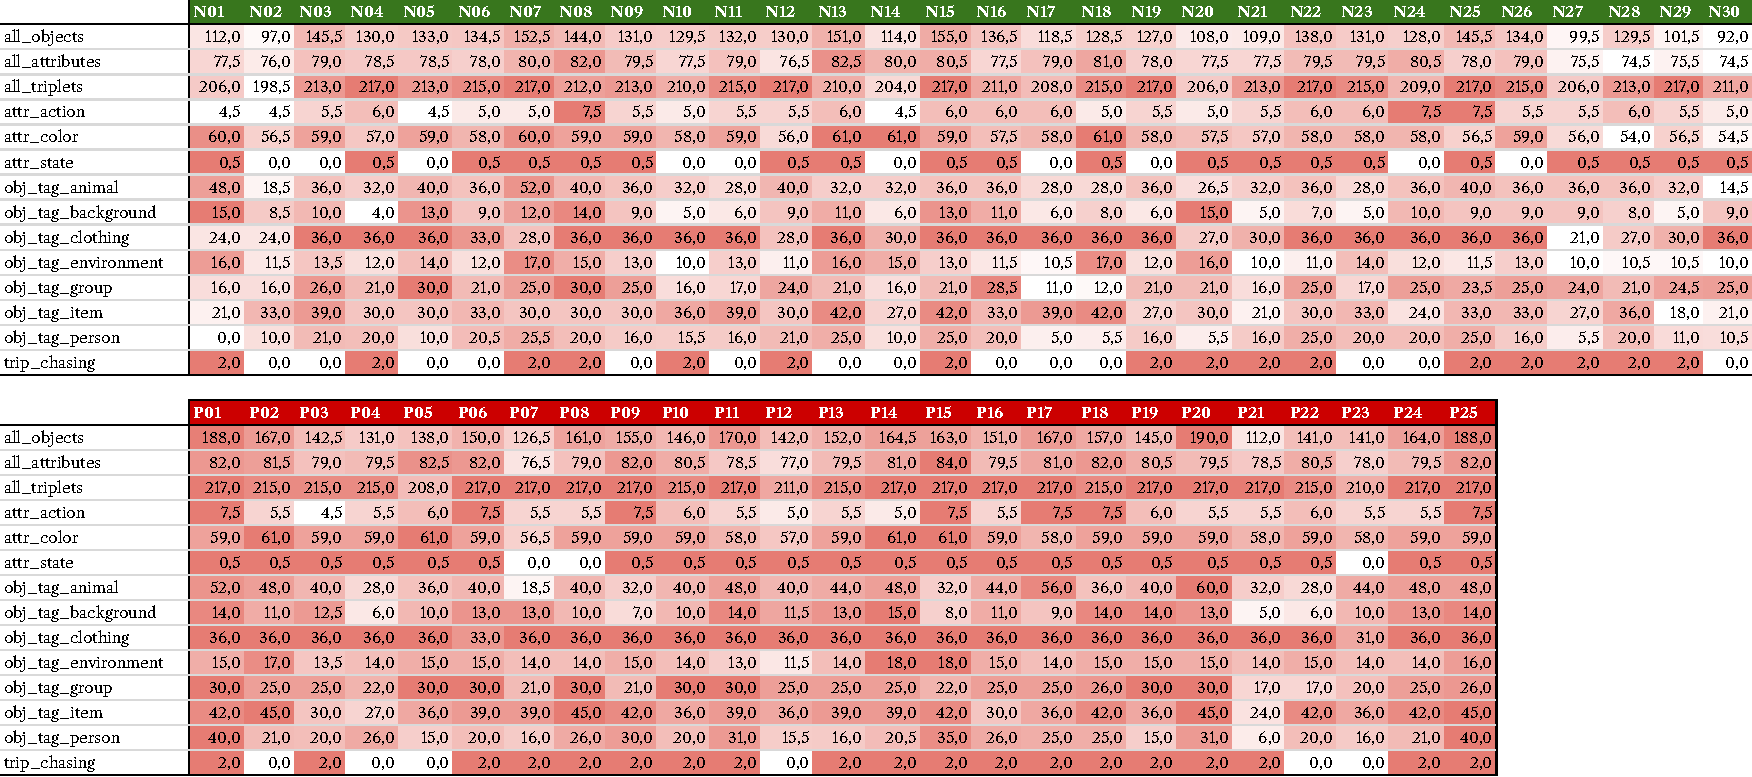
\includegraphics[width=0.86\paperheight]{./src/imgs/merged_v2.pdf}
		\caption{Vizuální znázornění rozdílných ztrát pro bez osoby bez diagnózy (sloupce \emph{N01} až \emph{N30}) a diagnostikované pacienty (sloupce \emph{P01} až \emph{P25})}\label{tab:color_table}
	\end{table}
\end{landscape}
\restoregeometry

